\section{Implementácia} \label{sec_kick_implementation}

\subsection{Vytvorenie prvého kopu do strany} \label{sec_lle2_kick_impl}

V kapitole \ref{sec_lle2} sme získali závislosť natočenia kĺbu \texttt{LLE2} od želanej hodnoty smeru uhla $\alpha$ vyjadrenej rovnicou \ref{eq_lle2}. 

Na základe tohto experimentu sme implementovali kop do strany. Na vstupe je uhol smeru lopty. Pri vykonaní kopu upravíme fázu 5 pohybu 
\newline\texttt{kick\_left\_normal\_stand}, resp. \texttt{kick\_right\_normal\_stand}. V tejto fáze sa nastaví vypočítané natočenie kĺbu \texttt{LLE2}. V prípade, že vypočítaná hodnota natočenia kĺbu sa nachádza mimo intervalu $<15;45>$, bude nastavená na hraničné hodnoty. Implementácia sa nachádza v triede \texttt{DirectionalKick}.

\subsection{Kop s posunom hráča do strany} \label{sec_kick_step_impl}

Pre dosiahnutie kopu podľa kapitoly \ref{sec_foot_biliard} sme testovali pohyb \newline\texttt{kick\_left\_very\_small}, aby sme zistili, o akú vzdialenosť sa hráč posunie do strany. Hráča sme umiestnili na pozíciu $[-0,2; -0,55; 0,4]$ a nechali ho pohyb vykonať 10-krát. Do tabuľky sme zapísali pozíciu hráča. Hodnoty sme zapísali do tabuľky a vypočítali priemernú hodnotu posunu. 

Rovnakým spôsobom sme vypočítali posun do strany pre pohyb \newline\texttt{kick\_left\_small}. Priebehy experimentov sa nachádzajú v prílohe v súbore \newline\texttt{experiment\_step\_left.ods} a výsledné priemerné posuny boli:
\begin{itemize}
	\item $0,0152~m$ pre \texttt{kick\_left\_very\_small}
	\item $0,0514~m$ pre \texttt{kick\_left\_small}
\end{itemize}

Rovnaké vzdialenosti platia aj pre symetrické pohyby do pravej strany \newline\texttt{kick\_right\_very\_small} a \texttt{kick\_right\_small}

Na základe získaných vzdialeností posunu hráča a rovnice \ref{eq_alfa_dependent_y_shift} sme vytvorili pohyb, ktorý na základe želaného uhla smeru lopty vypočíta počet posunov hráča do strany a vykoná pohyb spoločne s kopom. Implementácia sa nachádza v triede \texttt{DirectionalKickStep}.

\subsection{Kop s variabilným posunom hráča do strany} \label{sec_var_shift_kick_impl}
Z kapitol \ref{sec_foot_biliard}, \ref{sec_max_fixed_joints}, \ref{sec_fix_15_shift} a \ref{sec_fix_15_shift} vyplýva, že je možné dosiahnuť ešte väčší uhol konečnej pozície lopty ako pri kope opísaným z kapitoly \ref{sec_lle2} a \ref{sec_lle2_kick_impl}. A to vtedy, keď je pred kopom vykonaný posun hráča do ľavej, resp. pravej strany. Posun hráča do strany vykonávajú staticky definované pohyby \texttt{step\_left}, \texttt{step\_left\_small} a \texttt{step\_left\_very\_small} do ľavej strany. Resp. pre pravú stranu \texttt{step\_right}, \texttt{step\_right\_small} a \texttt{step\_right\_very\_small}. Tieto pohyby predstavujú posun do strany o $3$ rôzne vzdialenosti.

Každý z týchto pohybov sa skladá z troch fáz a líšia sa len vo fáze $2$. Pre posun do ľavej strany nastáva jediná zmena, a to v kĺbe \texttt{RLE2}. Do pravej strany zmena nastáva pri kĺbe \texttt{LLE2}. Z toho vyplýva, že existuje závislosť vzdialenosti posunu hráča do strany a veľkosti natočenia kĺbu \texttt{LLE2} (\texttt{RLE2}). 

Pri určovaní závislosti sme hráča umiestnili na pozíciu $[-0,2;0]$ a menili natočenie kĺbu \texttt{RLE2} o $5^{\circ}$, pohyb vykonali 10-krát, namerali vzdialenosť posunu a vypočítali priemer hodnôt.

Priemerné namerané hodnoty posunov zobrazuje tabuľka \ref{tab_step_left_RLE2}, kde \texttt{RLE} predstavuje natočenie kĺbu a $\bar{d_y}$ priemernú vzdialenosť posunu hráča na osi $y$ ihriska. Kompletné merania sa nachádzajú v priloženom súbore \newline\texttt{experiment\_steps\_left.ods}.

\begin{table}[H]
	\centering
	\footnotesize
	\begin{tabular}{||l||r|r|r|r|r|r|r|r|r|r||}
		\hline
		\hline
		$RLE2~(^{\circ})$ & $0$ & $-5$ & $-10$ & $-15$ & $-20$ & $-25$ & $-30$ & $-35$ & $-40$ & $-45$ \\
		\hline
		$\bar{d_y}~(m)$ & $0$ & $-0,002$ & $0,032$ & $0,027$ & $0,045$ & $0,051$ & $0,099$ & $0,11$ & $0,098$ & $0,091$ \\
		\hline
		\hline
	\end{tabular}
	\caption{Priemerné hodnoty posunu do ľavej strany pri meniacom natočení kĺbu \texttt{RLE2}}
	\label{tab_step_left_RLE2}
\end{table}

Ak položíme želaný posun hráča na os $x$ a hodnoty natočenia kĺbu \texttt{RLE2} na os $y$, dostaneme takú závislosť, ktorú zobrazuje graf na obrázku \ref{pic_dependency_RLE2_to_step_left}. Závislosť posunu a kĺbu je vyjadrená rovnicou trendovej čiary \ref{eq_dependency_RLE2_to_step_left}.

\begin{figure}[H]
	\centering
	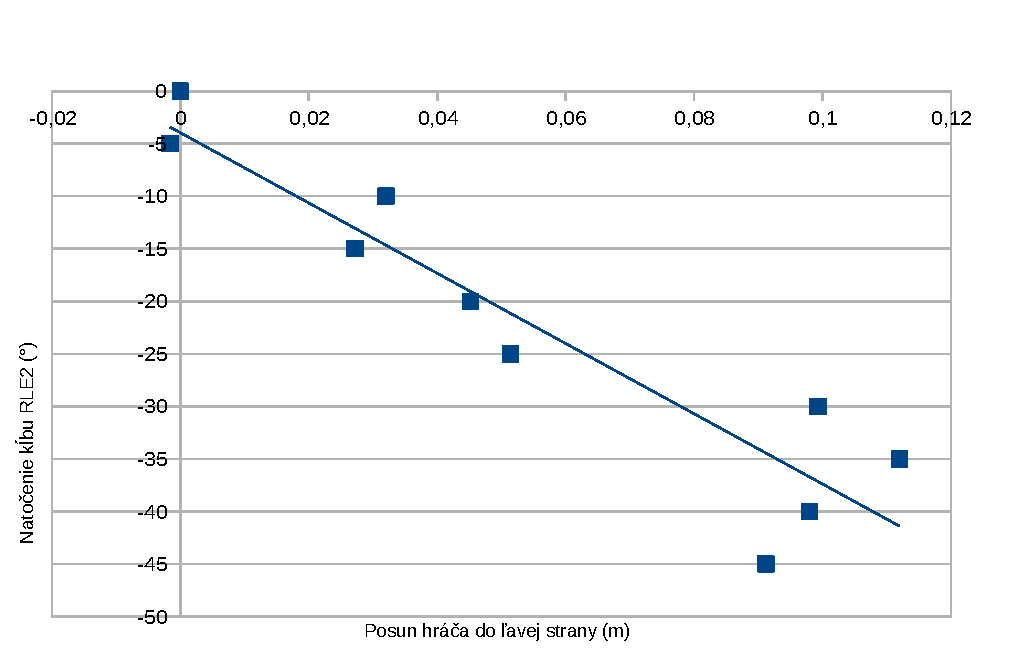
\includegraphics[scale=0.7]{./data/dependency_RLE2_to_step_left}
	\caption{Závislosť natočenia kĺbu RLE2 od vzdialenosti posunu hráča do ľavej strany}
	\label{pic_dependency_RLE2_to_step_left}
\end{figure}

\begin{equation} \label{eq_dependency_RLE2_to_step_left}
	f_l(x) = -334,2834552537x - 3,9572967371
\end{equation}

Pre závislosť úkroku do pravej strany pre kĺb \texttt{LLE2} platí: 
\begin{equation}
	f_r(x) = -f_l(x)
\end{equation}


Túto vlastnosť sme využili pri úprave pohybu \texttt{DirectionalKickStep}. Namiesto šliapania do strany niekoľkokrát za sebou môžeme vykonať jeden veľký úkrok a následne vykonať kop. Týmto spôsobom sme vytvorili druhú implementáciu pohybu, ktorý sa nachádza v triede \texttt{DirectionalKickStepV2}.

\subsection{Kopy s variabilným posunom hráča do strany a zafixovaním kĺbu \texttt{LLE2}} \label{sec_var_shift_fixed_joint_kick_impl}
Implementáciu nasledujúcich dvoch kopov sme vytvorili využitím rovníc \ref{eq_lle2_15_y_shift}  a \ref{eq_lle2_45_y_shift}, ktoré opisujú uhol smeru lopty s posunom hráča do strany a zafixovaní kĺbu \texttt{LLE2}. Najprv sa vykoná variabilný posun rovnako ako v kapitole \ref{sec_var_shift_kick_impl} a následne vo fáze 5 kopu sa nastaví hodnota kĺbu \texttt{LLE2} na 15, resp. 45.

Tieto 2 kopy sú implementované v triedach \texttt{DirectionalKickStepV3} a \texttt{DirectionalKickStepV4}

\subsection{Implementácia modulu inverznej kinematiky} \label{sec_implementation}

Aby fakultný robot dokázal využívať pohyby vypočítané inverznou kinematikou, opísané v kapitole \ref{sec_specification}, rozhodli sme sa výpočet, čo najviac oddeliť od súčasnej štruktúry kódu. Ako podklad sme si zvolili implementáciu diplomovej práce Pavla Meštaníka, ktorá je opísaná v kapitole \ref{sec_mestanik}. Vznikol tak samostatný balíček v jazyku Java s menom \texttt{sk.fiit.jim.agent.moves.kinematics}. 

Súčasťou sú tieto triedy:
\begin{itemize}
	\item \texttt{ForwardKinematicResult}
	\item \texttt{HeadIk}
	\item \texttt{Kinematics}
	\item \texttt{KinematicUtils}
	\item \texttt{LeftArmIk}
	\item \texttt{LeftLegIk}
	\item \texttt{Matrix}
	\item \texttt{Orientation}
	\item \texttt{RightArmIk}
	\item \texttt{RightLegIk}
	\item \texttt{SimsparkConstants}
\end{itemize}

Triedy \texttt{Kinematics}, \texttt{Matrix}, \texttt{Orientation} sú jediné, ktoré sú viditeľné aj v iných balíčkoch, ostatné sú viditeľné len v rámci nového balíka. V nasledujúcej kapitole \ref{sec_classes_desc} si popíšeme funkcionalitu každej triedy.

\subsection{Popis tried} \label{sec_classes_desc}
\textbf{Trieda \texttt{Kinematics}}
\\
Táto trieda obsahuje metódy, ktoré slúžia na vrátenie výsledkov výpočtov pre doprednú a inverznú kinematiku popísaných rovnicami z kapitoly \ref{sec_specification} pre všetky 4 končatiny (ľavú, resp. pravú ruku a ľavú, resp. pravú ruku). Výpočet pre hlavu sa momentálne nevyužíva.
\\\\
\textbf{Trieda \texttt{Matrix}}
\\
Slúži sa na maticové operácie, ktoré sa využívajú pri doprednej a inverznej kinematike. Zároveň obsahuje niektoré matice ako konštanty, ktoré sa často využívajú pri výpočtoch. 
\\\\
\textbf{Trieda \texttt{Orientation}}
\\
Úlohou tejto triedy je zapuzdriť natočenie koncového efektora podľa zodpovedajúcich osí $x$, $y$, $z$.
\\\\
\textbf{Triedy \texttt{LeftArmIk}, \texttt{LeftLegIk}, \texttt{RightArmIk}, \texttt{RightLegIk}, \texttt{HeadIk}}
\\
Obsahujú výpočty pre uhly zodpovedajúcim končatinám.
\\\\
\textbf{Triedy \texttt{SimsparkConstants}, \texttt{KinematicUtils}}
\\
Pomocné triedy na uchovávanie konštánt a pomocných metód pre všetky ostatné výpočty.
\\\\
\textbf{Ostatné triedy}\\
Zároveň boli rozšírené existujúce balíčky novými triedami. Tie slúžia na využije inverznej kinematike pri pohyboch robota. Nové triedy:
\begin{itemize}
	\item \texttt{DynamicMove} - slúži ako predloha pre dynamické pohyby. Vstupom je sekvencia pozícií a natočení koncového vektora zodpovedajúcej končatiny.
	\item \texttt{DirectionalKick} - implementácia kopu podľa kapitoly \ref{sec_lle2_kick_impl}
	\item \texttt{DirectionalKickStep} -  implementácia kopu podľa kapitoly \ref{sec_kick_step_impl}
	\item \texttt{DirectionalKickStepV2} - implementácia kopu podľa kapitoly \ref{sec_var_shift_kick_impl}
	\item \texttt{DirectionalKickStepV3} - implementácia kopu podľa kapitoly \ref{sec_var_shift_fixed_joint_kick_impl}
	\item \texttt{DirectionalKickStepV4} - implementácia kopu podľa kapitoly \ref{sec_var_shift_fixed_joint_kick_impl}
\end{itemize}

Závislosti medzi triedami a balíčkami sú zobrazené na obrázku \ref{pic_class_diagram}. Obrázok neobsahuje všetky triedy, ale len relevantné pre opis implementácie. Novovytvorené triedy a balíčky sú zvýraznené tmavou farbou.

\begin{landscape}
\thispagestyle{empty}
\newgeometry{right=-8cm} % magické číslo, aby to bolo pekne zarovnané.
\begin{figure}[H]
\centering
	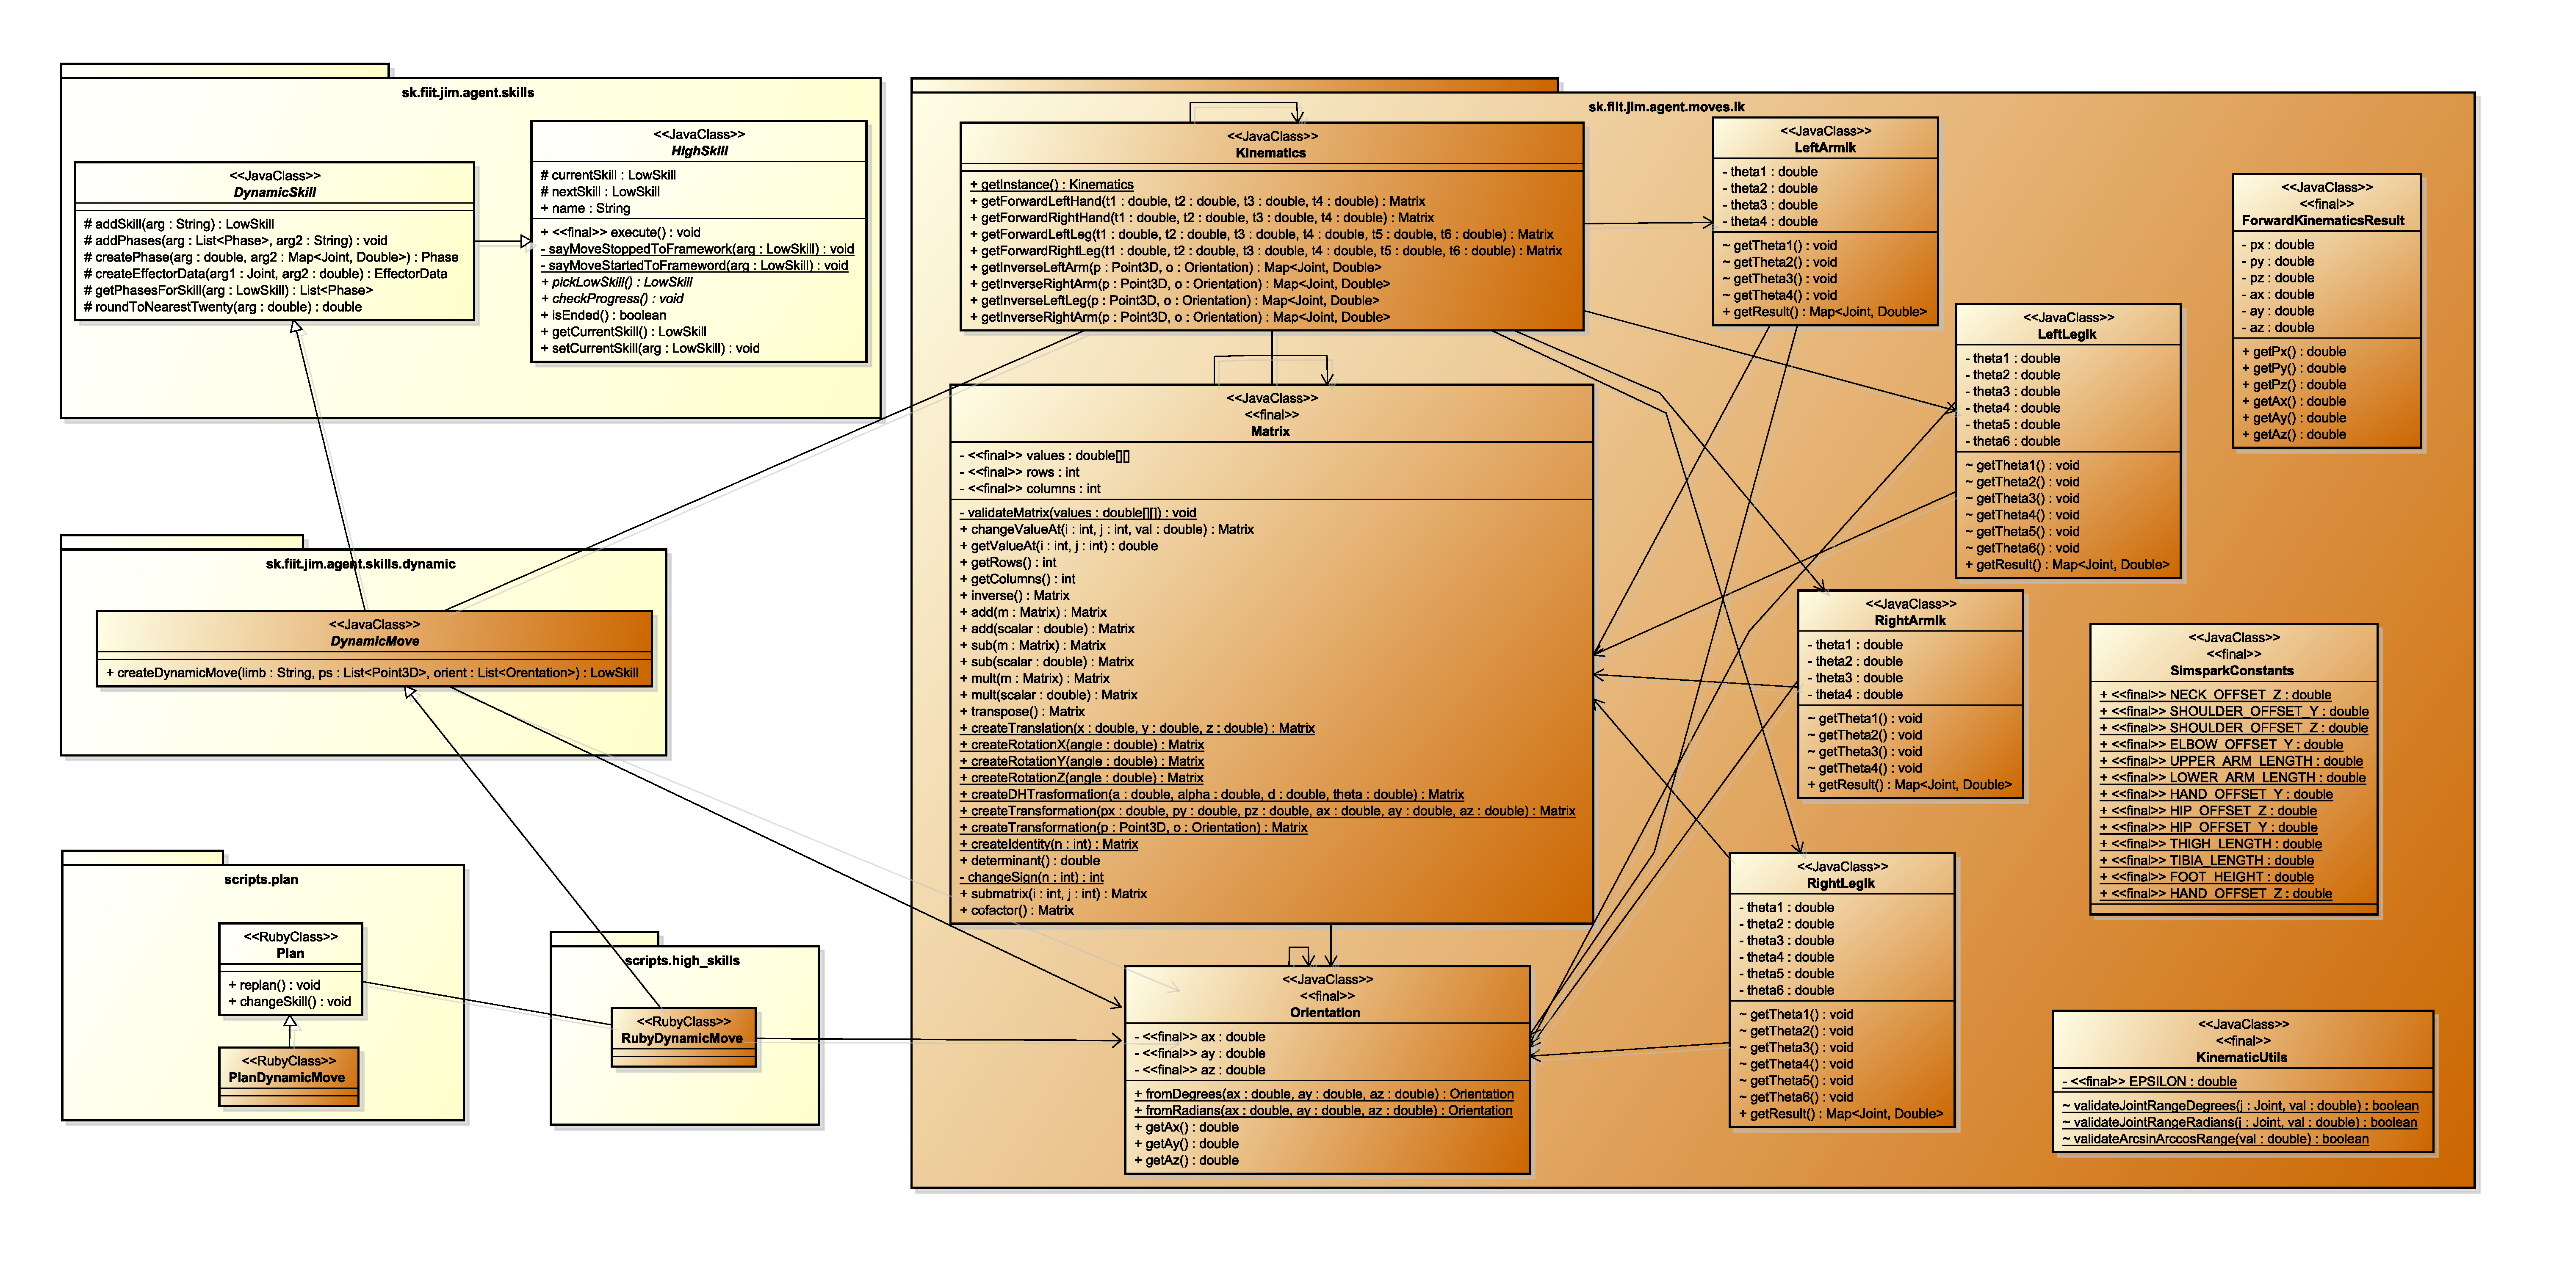
\includegraphics[scale=0.28]{./data/class_diagram}
	\caption{Diagram tried vytvoreného modulu inverznej kinematiky a nových pohybov}
	\label{pic_class_diagram}
\end{figure}
\end{landscape}

